
\documentclass{report}

\usepackage[english,ngerman]{babel} 
\usepackage[utf8]{inputenc} 
\usepackage{graphicx}
\usepackage{dsfont}
\usepackage{amsmath}

\title{TH1 - Aufgabenblatt 1}
\author{Andreas Krohn, Erik Andresen, Benjamin Vetter}

\begin{document}

\maketitle

\begin{enumerate}
\item Modelliert einen einfachen Fahrstuhl für 3 Stockwerke, der immer fährt, bis ganz oben (3) und dann wieder bis ganz unten (1).

\item Fügt die Halte-Anforderung für jedes Stockwerk hinzu. Wenn eine Halte-Anforderung vorliegt, hält der Fahrstuhl und die Türen werden geöffnet und vor der Weiterfahrt geschlossen.

\item Modelliert nun einen Fahrstuhl mit einer einfachen Steuerung. Der Fahrstuhl fährt nur, wenn eine Anforderung vorliegt. Falls eine Anforderung für das Stockwerk, in dem sich der Fahrstuhl gerade befindet, vorliegt, werden die Türen geöffnet und anschließend geschlossen. Es wird immer nur eine Anforderung bearbeitet, d.h. Anforderungen werden nicht angenommen, wenn der Fahrstuhl gerade arbeitet.

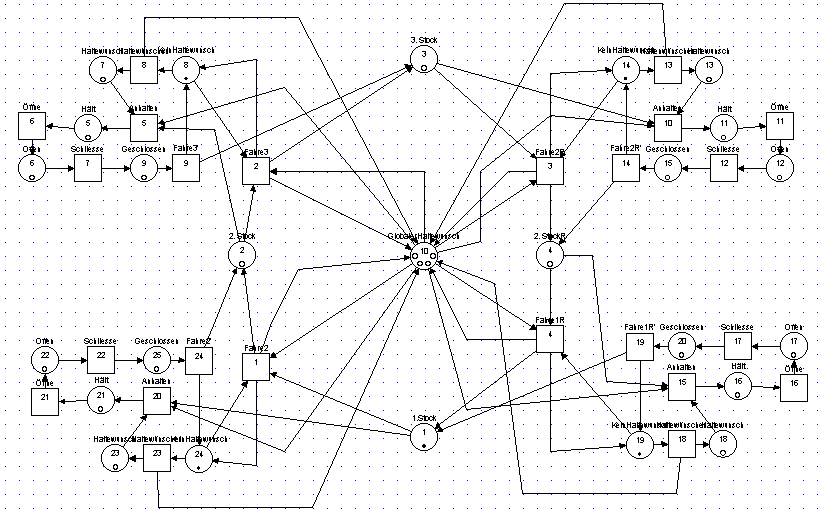
\includegraphics[width=1\textwidth]{graph.png}

\item Gebt das Netz formal in klassischer Darstellung an.

$N = (P, T, W, K, M_0)$

$P_1 = \{ 1Stock, 2Stock, 3Stock, 2StockR, GlobalerHaltewunsch \}$

$P_2 = \bigcup_{i \in \{ 1, 2, 2R, 1R \}} \{ Haltewunsch_i, KeinHaltewunsch_i, H"alt_i, Offen_i, Geschlossen_i \}$

$P = P_1 \cup P_2$

Es gilt:

$
1Stock < 2Stock < 3Stock < 2StockR < GlobalerHaltewunsch 
< Haltewunsch_1 < KeinHaltewunsch_1 < H"alt_1 < Offen_1 < Geschlossen_1
< Haltewunsch_2 < KeinHaltewunsch_2 < H"alt_2 < Offen_2 < Geschlossen_2
< Haltewunsch_2R < KeinHaltewunsch_2R < H"alt_2R < Offen_2R < Geschlossen_2R
< Haltewunsch_1R < KeinHaltewunsch_1R < H"alt_1R < Offen_1R < Geschlossen_1R
$

$T = \bigcup_{i \in \{ 1, 2, 2R, 1R \}} \{ Fahre_i, Fahre_i', Haltew"unschen_i, Anhalten_i, "Offne_i, Schliesse_i \}$

$W : (P \times T) \cup (T \times P) \rightarrow \mathds{N}_0$

$\forall (x, y) \in (P \times T) \cup (T \times P): W(x,y) = 1$

$K : P \rightarrow \mathds{N}_0$

$
K(p) = 
  \begin{cases}
    3, & \text{falls $p \in \{ GlobalerHaltewunsch \}$} \\ 
    1, & \text{sonst} \end{cases}$

$
M_0 = (1, 0, 0, 0, 0, 
0, 1, 0, 0, 0,
0, 1, 0, 0, 0,
0, 1, 0, 0, 0,
0, 1, 0, 0, 0)
$

\end{enumerate}

\end{document}

